\documentclass[../TDE1-E2.tex]{subfiles}%

\begin{document}
\section[s]"2"{Diviseur de courant}

\enonce{%
    \begin{center}
  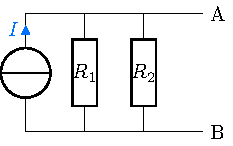
\includegraphics[scale=1]{divcour_plain}
\end{center}
}%

\QR{%
  Exprimer les tensions aux bornes de $R_1$ et $R_2$ dans le montage
        ci-contre.
}{%
\vspace{-15pt}
\begin{tcbraster}[raster columns=3, raster equal height=rows]
    \begin{tcn}(data){Schéma}
        \begin{center}
            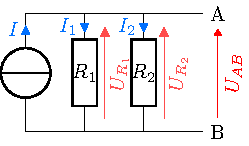
\includegraphics{divcour}
        \end{center}
    \end{tcn}
    \begin{tcolorbox}[blankest, raster multicolumn=1, space to=\myspace]
        \begin{tcbraster}[raster columns=1]
            \begin{tcn}(ques)""{Résultat attendu}
                On cherche $U_{R_1}$ et $U_{R_2}$.
            \end{tcn}
            \begin{tcn}[add to natural height=\myspace](tool)""{Outils}
                \begin{itemize}
                    \item Unicité de la tension en parallèle~;
                    \item Expression résistance $\parr$.
                \end{itemize}
            \end{tcn}
        \end{tcbraster}
    \end{tcolorbox}
    \begin{tcn}(impl)"limp"'r'{Schéma simplifié}
        \begin{center}
            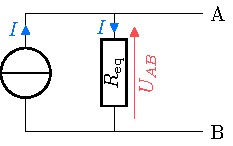
\includegraphics{divcour-simple}
        \end{center}
    \end{tcn}
\end{tcbraster}
\begin{tcbraster}[raster columns=2, raster equal height=rows]
    \begin{tcn}(appl){Application}
        On a certes $U_{R_1} = I_1R_1$ et $U_{R_2} = I_2R_2$, mais comme on a
        $U_{R_1} = U_{R_2} = U_{AB}$, le plus simple est de déterminer $U_{AB}$.
        Une résistance équivalente $R_{\rm eq} = \frac{R_1R_2}{R_1+R_2}$ avec
        l'intensité $I$ qui est connue (car imposée par le générateur de
        courant) donne facilement \[U_{R_1} = U_{R_2} = R_{\rm eq}I =
        \frac{R_1R_2}{R_1+R_2}I\]
    \end{tcn}
    \begin{tcn}(ror)'r'{Important}
        Ce résultat est la base de la réflexion menant à l'expression du
        diviseur de courant qui donne l'expression de $I_x$~: on voit
        directement apparaître que $\DS I_x = I\times\frac{R_{\rm eq}}{R_x}$ de par
        l'unicité de la tension. Souvenez-vous de cette simplicité.
    \end{tcn}
\end{tcbraster}
}%
\QR{%
  À partir de la loi des mailles, exprimer $I(R_2$) en fonction de I,
        $R_1$ et $R_2$.
}{%
\vspace{-15pt}
\begin{tcbraster}[raster columns=3, raster equal height=rows]
    \begin{tcn}(ques){Résultat attendu}
        On cherche $I_2$ en fonction de $I, R_1, R_2$ \textbf{à partir de la loi
        des mailles}.
    \end{tcn}
    \begin{tcn}(tool)""{Outils}
        -- LdM~: $I_1R_1 = I_2R_2 \quad \color{ForestGreen}(1)$~;
        \smallbreak
        -- LdN~: $I = I_1 + I_2 \quad \color{ForestGreen}(2)$.
    \end{tcn}
    \begin{tcn}(appl)'r'{Application}
        En utilisant \textcolor{ForestGreen}{(2)} dans
        \textcolor{ForestGreen}{(1)}, on a $I_2R_2 = (I-I_2)R_1$, donc en
        isolant $I_2$ on obtient facilement \[\boxed{I_2 = I
        \frac{R_1}{R_1+R_2}}\]
    \end{tcn}
\end{tcbraster}
}%

\enonce{%
  On ajoute une résistance $R_3$ qui sera connectée en parallèle avec la
résistance $R_1$.
}%

\QR{%
  Faire un schéma. Est-ce que la valeur de l'intensité $I(R_2$) va changer~?
  Si oui, donner sa nouvelle expression.
}{%
\vspace{-15pt}
\begin{tcbraster}[raster columns=7, raster equal height=rows]
    \begin{tcolorbox}[blankest, raster multicolumn=4, space to=\myspace]
        \begin{tcbraster}[raster columns=1]
    \begin{tcn}(data){Schéma}
        \begin{center}
            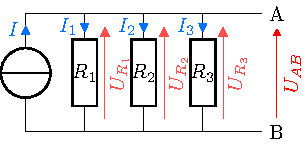
\includegraphics{divcour_3}
        \end{center}
    \end{tcn}
    \begin{tcn}(ques){Résultat attendu}
        Évidemment, $I_2$ va changer puisqu'on branche un nouveau dipôle en
        parallèle. Une rivière qui se divise en 3 plutôt qu'en 2 va avoir des
        débits différents dans les deux situations. Donc on cherche $I_2$ en
        fonction de $I, R_1, R_2, R_3$ \textbf{sans méthode imposée}.
    \end{tcn}
        \end{tcbraster}
    \end{tcolorbox}
    \begin{tcn}[raster multicolumn=3](appl)'r'{Application}
        Avec la réflexion de la question 1 ou la relation du pont diviseur de
        courant qui est maintenant utilisable à volonté, on a facilement $I_2 =
        I\times \frac{R_{\rm eq}}{R_2}$. Avec $R_{\rm eq} =
        \frac{R_1R_2R_3}{R_1R_2+R_1R_3+R_2R_3}$, on a finalement
        \[\boxed{I_2 = I \times \frac{R_1R_3}{R_1R_2+R_1R_3+R_2R_3}}\]
    \end{tcn}
\end{tcbraster}
}%

\QR{%
  Est-ce que la valeur de l'intensité délivrée par le générateur va
        changer~? Si oui, donner sa nouvelle expression.
}{%
\vspace{-15pt}
\begin{tcbraster}[raster columns=2, raster equal height=rows]
    \begin{tcn}(rema){Remarque}
        L'intensité $I$ ne va pas changer, puisque c'est celle que l'on fixe
        avec le générateur.
    \end{tcn}
    \begin{tcn}(ror)'r'{Important}
        Bien que la loi des mailles soit l'origine de nombreuses relations, ici
        c'est la simple unicité de la tension qui amène au diviseur de courant.
    \end{tcn}
\end{tcbraster}
}%

\end{document}
